%==============================================================================
\section{Results for the Baseline Geometry}
\label{sec:results_baseline}
%==============================================================================

\begin{table}[htpb]
 \caption{Uncertainties on all systematic parameters for the baseline
  detector model with three years of lifetime, ranked according to their impact
  on the mass hierarchy parameter $h$.}
 \label{tab:baseline_results}
 \begin{center}
  \small{\begin{tabular}{lrrrrrr} 
\toprule
Parameter & Impact [\%] & Best Fit & $\sigma^\mathrm{full}$ & $\sigma^\mathrm{stat}$ & $\sigma^\mathrm{syst}$ & Prior \\ 
\midrule
$h$ & 100.0 & \num{1.00e+00} & \num{3.43e-01} & \num{2.33e-01} & \num{2.52e-01} & free \\
$r_{A_\mathrm{eff},\,\nu-\bar\nu}$ & 8.9 & \num{0.00e+00} & \num{4.73e-02} & \num{4.76e-03} & \num{1.47e-01} & \num{5.00e-02} \\
$\vartheta_{13}$ [$^\circ$] & 8.0 & \num{8.93e+00} & \num{4.64e-01} & \num{8.24e-01} & \num{3.67e+00} & \num{4.68e-01} \\
$n_{A_\mathrm{eff}}$ & 7.4 & \num{0.00e+00} & \num{1.94e-02} & \num{1.99e-03} & \num{1.94e-02} & \num{2.00e-01} \\
$\vartheta_{23}$ [$^\circ$] & 3.2 & \num{3.86e+01} & \num{4.67e-01} & \num{3.02e-01} & \num{3.97e-01} & \num{1.32e+00} \\
$\Delta m^2_{31}$ [eV$^2$] & 2.7 & \num{2.46e-03} & \num{6.49e-05} & \num{1.77e-05} & \num{1.10e-04} & \num{8.00e-05} \\
$r_{\Phi,\,\nu_e-\nu_\mu}$ & 2.4 & \num{0.00e+00} & \num{1.10e-02} & \num{5.12e-03} & \num{1.01e-02} & \num{5.00e-02} \\
$s_{A_\mathrm{eff}}$ [m$^2$/GeV] & 1.1 & \num{0.00e+00} & \num{2.19e-04} & \num{1.23e-04} & \num{1.82e-04} & free \\
$\Delta_\mathrm{PID}$ [GeV] & 0.9 & \num{0.00e+00} & \num{1.70e-02} & \num{1.58e-02} & \num{6.23e-03} & \num{5.00e-01} \\
$s_E$ & 0.1 & \num{1.00e+00} & \num{2.81e-02} & \num{7.66e-03} & \num{3.31e-02} & \num{5.00e-02} \\
\bottomrule 
\end{tabular}
}
 \end{center}
\end{table}

Using the settings described in the previous section, the Fisher matrix for
PINGU can now be constructed with \papa. The full, statistical, and systematic
errors are for all parameters are listed in Tab.~\ref{tab:baseline_results} for
a nominal PINGU lifetime of three years. The parameters are ordered after their
\emph{impact} on the mass hierarchy parameter $h$, which is defined as the
square of their correlation coefficient $c_{ih}$ (\ref{eqn:corr_coeff}) with
$h$. Note that for the baseline settings, the systematic parameter
$s_\mathrm{PID}$ has been excluded as it is fully degenerate with $n_{\aeff}$:
since the PID decision is binary, no channel of unidentified events exists and
hence both parameters just evenly increase the overall number of events,
effectively.

From the first line of Tab.~\ref{tab:baseline_results}, one can read off the
expected significance of PINGU's mass hierarchy measurement by inverting the
full error (see Sec.~\ref{sec:fisher_hierarchy}). This gives an expected
significance of 2.9\,$\sigma$ after three years. Looking at the statistical
error alone, this value increases to 4.3\,$\sigma$, emphasising the important
role systematic parameters are playing in the determination of the mass
hierarchy.

\begin{figure}[bhtp]
 \centering
 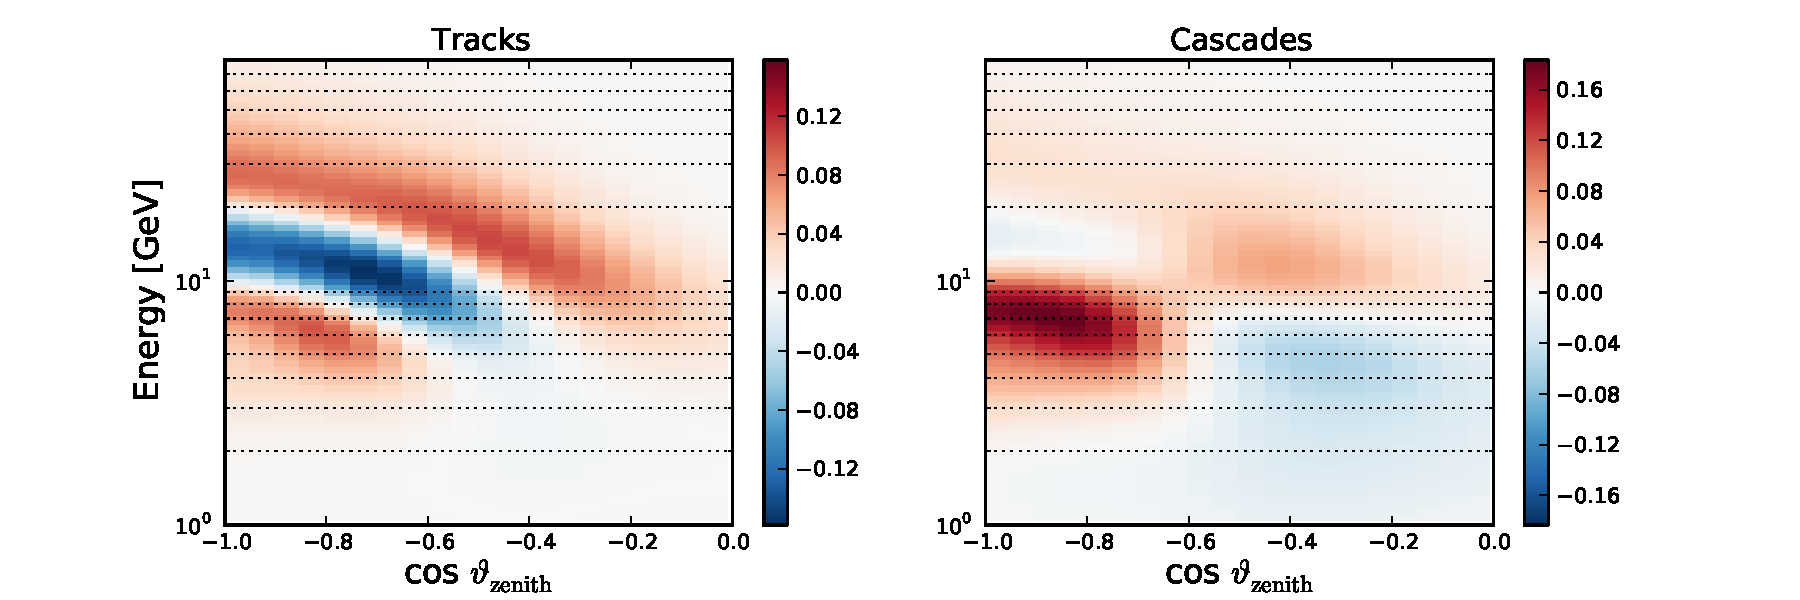
\includegraphics[width=\linewidth]{akhmedov_baseline}
 \caption{\delchi distribution in the track (left) and cascade (right) channels 
for the baseline settings.}
 \label{fig:akhmedov_baseline}
\end{figure}

\begin{figure}[thp]
 \centering
  \subfloat[\label{fig:sigma_vs_time}]
   {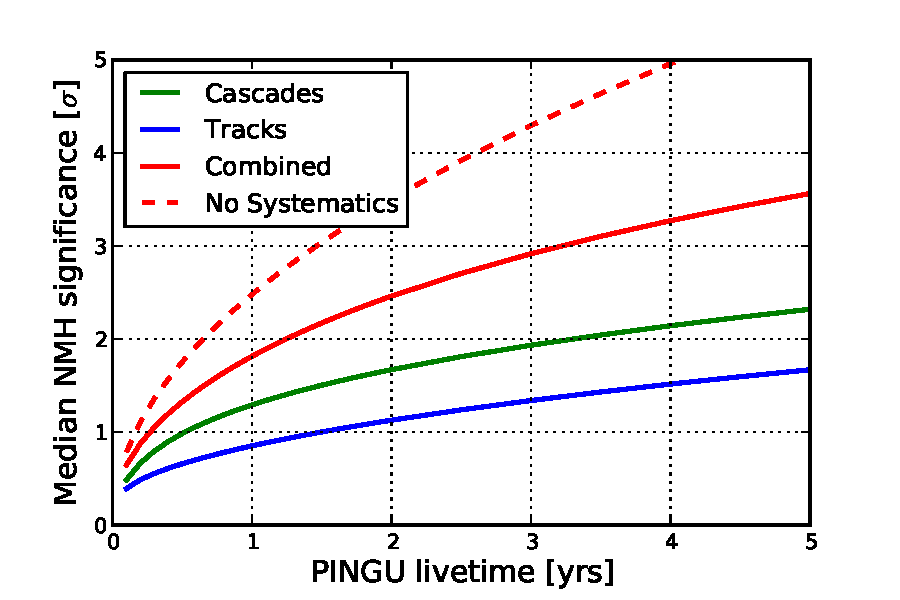
\includegraphics[width=0.495\linewidth]{sigma_vs_time_default}}
  \subfloat[\label{fig:covmat_baseline}] 
   {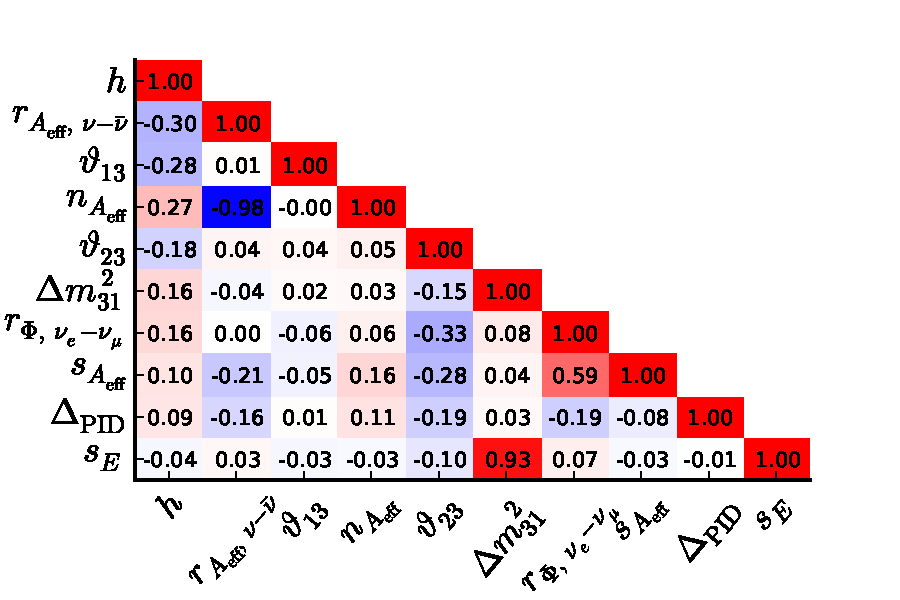
\includegraphics[width=0.495\linewidth]{CovMat_PINGU}}
 \caption{\protect\subref{fig:sigma_vs_time} Evolution of PINGU's expected mass 
          hierarchy significance with time and 
          \protect\subref{fig:covmat_baseline} Full correlation matrix for PINGU
          for the baseline settings.}
 \label{fig:time_covmat}
\end{figure}

Treating the track and cascade channels separately, the expected significances
are 1.9\,$\sigma$ with and 3.0\,$\sigma$ without systematics for the cascade
and 1.3\,$\sigma$ (3.1\,$\sigma$) for the track channel,
respectively\footnote{The full error listings corresponding to
Tab.~\ref{tab:baseline_results} can be found in
App.~\ref{app:fisher_baseline}}. Although the purely statistical significances
are comparable, when taking systematics into account the significance for the
cascades remains much higher than the track significance. 
The reason for this becomes obvious when looking at the \delchi distributions 
for both channels in Fig.~\ref{fig:akhmedov_baseline}. In the track channel, 
there are three distinct regions driving the expected significance. These 
regions are separated only by small margins and have alternating sign, while in 
the cascade channel most of the significance comes from one contiguous region. 
Together with the fact that the cascade channel has roughly three times higher 
event statistics than the track channel---62,000 vs.\ 22,000 neutrino events 
per year---this makes the cascade channel much more robust against the impact 
of systematic parameters.

In Fig.~\ref{fig:sigma_vs_time}, the significances for the individual channels 
and for their combination are shown as a function of time. The purely 
statistical significance is plotted as well, exhibiting a scaling with the 
square root of the lifetime as one would expect for a counting experiment where 
the relative error is proportional to $1/\sqrt{N}$. The actual significances 
including systematics increase much slower with time as a part of the 
accumulating statistics has to be ``spent'' in order to better constrain the 
systematic parameters. However the combined analysis of the two channels still 
gives a much higher sensitivity than simply adding the two individual channels 
in quadrature as one would do for two completely unrelated measurements of the 
same quantity. E.\,g.\ for a lifetime of three years as above, the quadratic 
sum of the track and cascade significances is $\sqrt{(1.3\,\sigma)^2 + 
(1.9\,\sigma)^2} \approx 2.3\,\sigma$, considerably lower than the 
2.9\,$\sigma$ for the combined analysis.

Finally one can look at the correlation matrix of PINGU. In contrast to the 
error listing for all parameters as in Tab.~\ref{tab:baseline_results}, here the 
interdependences between the parameters are in the focus. The graphical 
representation in Fig.~\ref{fig:covmat_baseline} shows, for every combination 
of parameters, their correlation coefficient $c_{ij}$. Using these quantities 
instead of the entries $\sigma_{ij}$ of the covariance matrix themselves has 
the benefit that due to their normalisation, cf.~(\ref{eqn:corr_coeff}), the 
entries of the matrix are dimensionless and restricted to the range $[-1, +1]$, 
thus making them easier to interpret.

From the correlation matrix itself, several things can be learned. First, the 
hierarchy parameter is the one with strongest overall correlations. This 
emphasises the fact that the determination of the neutrino mass hierarchy is a 
very delicate measurement relying on a small effect, and that the inclusion of 
so many systematic parameters is indeed necessary to get a robust result.

\begin{figure}[thp]
 \centering
 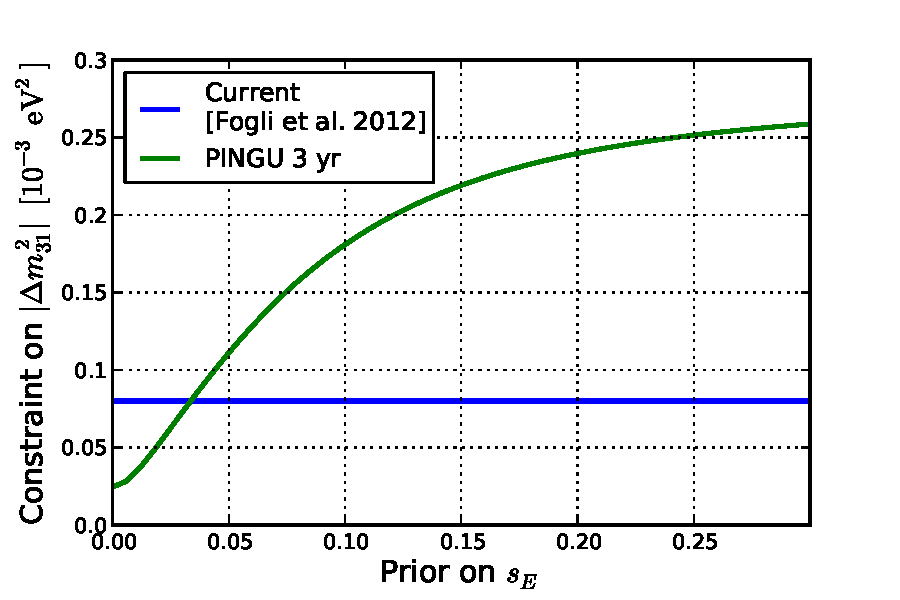
\includegraphics[width=0.7\linewidth]{dm31_vs_escale_prior}
 \caption{PINGU constraint on \dm{31} as a function of the prior on the energy
          scale. No prior knowledge about \dm{31} is assumed.}
 \label{fig:dm31_vs_escale_prior}
\end{figure}

Furthermore, two combinations of parameters stick out due to their very strong 
correlation. The first one is the relative normalisation of the effective areas 
for \nux and \nuxbar, $r_{\aeff,\,\nu-\bar\nu}$, and the overall normalisation 
of all effective areas, $n_{\aeff}$. Their anticorrelation is obvious from 
their definition: $r_{\aeff,\,\nu-\bar\nu}$ increases the number of neutrino 
events while decreasing the number of antineutrino events. Since PINGU cannot 
distinguish between those and the cross-section for neutrinos is higher 
approximately by a factor of two (see Fig.~\ref{fig:NuXsec_GeV}), the total 
number of events is increased, which can be compensated by decreasing 
$n_\aeff$. Only the MSW resonance oscillation causes an asymmetry between 
neutrinos and antineutrinos, such that the anticorrelation is not exactly $-1$.

The second strong correlation can be observed between the absolute value of the 
mass splitting \dm{31} and the energy scale $s_E$. The value of \dm{31} is 
determined from the position of the oscillation minimum in the track channel 
that is easy to spot in Fig.~\ref{fig:SimSteps}. In a two-flavour approximation, 
this can be described by equation (\ref{eqn:osc_length}), where the oscillation 
length is determined by the zenith angle. Then \dm{31} is inversely 
proportional to the neutrino energy. Thus a larger value of \dm{31} can be 
compensated by increasing the energy scale accordingly.

This means that if PINGU is supposed to make a precise measurement of \dm{31}, 
the energy scale has to be known very accurately. As the energy of a neutrino 
event is determined primarily from the number of detected photons\footnote{The 
Cherenkov light output is directly proportional to the deposited energy.}, this
means that the photon detection efficiency of the optical modules has to be
well calibrated. This behaviour is illustrated in
Fig.~\ref{fig:dm31_vs_escale_prior}, where PINGU's self-contained constraint on
the value of \dm{31} is plotted against the prior put on $s_E$. To improve on
the current limits, the energy scale has to be known with an accuracy of at
least 3\,\%.

\subsection{Measuring the Atmospheric Mixing Parameters}
\label{sec:results_atmosperic}

\begin{figure}[thp]
 \centering
 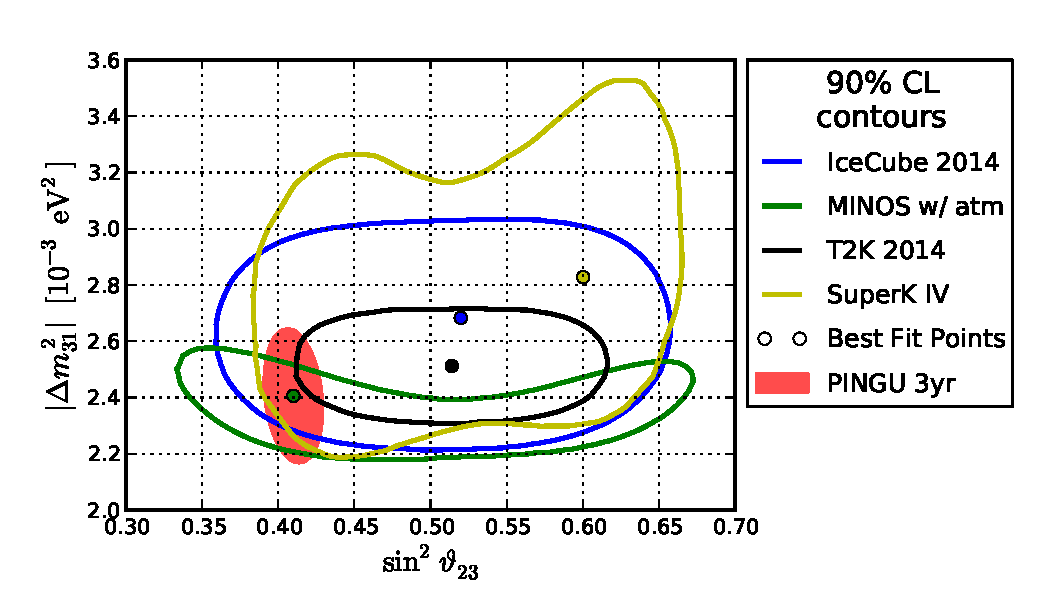
\includegraphics[width=0.85\linewidth]{AtmoParamsBaseline}
 \caption{PINGU constraint on \dm{31} and $\sin^2\thet{23}$ for the baseline
          settings. No prior knowledge about the two parameters is assumed.
          The latest constraints from the IceCube/DeepCore \cite{DCosc}, MINOS
          \cite{MINOSparams}, T2K \cite{T2Kparams}, and SuperKamiokande
          \cite{SuperKparams} are shown for reference.}
 \label{fig:AtmoParamsBaseline}
\end{figure}

To determine the neutrino mass hierarchy, PINGU makes a precision measurement
of the oscillations of atmospheric neutrinos. In fact, with more than 80,000
events recorded per year it will collect the largest sample of atmospheric
neutrinos so far. After DeepCore has been established as a serious contributor
to the global effort of characterising neutrino oscillations, PINGU will go
even further into that direction and provide tight constraints on the values of
\dm{31} and \thet{23}.

These constraints are shown in Fig.~\ref{fig:AtmoParamsBaseline}, along with
the most recent confidence regions of current oscillation experiments. For
PINGU, no priors have been put on \dm{31} or \thet{23}, meaning that the
displayed confidence ellipse comes from PINGU data alone and does not profit
from external knowledge.

The most obvious feature of PINGU's confidence ellipse is its orientation,
which is different from the other experiments: While it cannot constrain
\dm{31} any better than current experiments, the value of \thet{23} will be
much more precise than any measurement available today. The reason for this is
that the value of \dm{31} is extracted from the position of the oscillation
minimum in energy, which needs a precise calibration of the energy scale as we
have seen above. This is much easier to achieve in experiments on a neutrino
beam like MINOS or T2K where the beam energy is well-known. \thet{23} on the
other hand is determined from the relative depth of the oscillation minimum as
one can see from equation (\ref{eqn:twoflavour_prob}). Here PINGU profits from
its wide energy range including control regions without oscillations and the
large event statistics, such that especially the overall detector
efficiency\footnote{Represented by $n_\aeff$ in \papa.}, which usually is
difficult to constrain in beam experiments, only has minor impact.

\subsection{Impact of the Octant of \thet{23}}
\label{sec:results_octant}

\subsection{High-Purity Event Classification}
\label{sec:results_includeunkn}

\subsection{The Missing Monte Carlo Effect}
\label{sec:results_mcstats}

